\documentclass{beamer}
\mode<presentation>{}

\usepackage{amsmath}
\usepackage{graphicx}
\graphicspath{ {/Users/matthewdrury/Presentations/boosting-presentation-for-galvanize/plots/} }

\AtBeginSection[]{
  \begin{frame}
  \vfill
  \centering
  \begin{beamercolorbox}[sep=8pt,center,shadow=true,rounded=true]{title}
    \usebeamerfont{title}\insertsectionhead\par%
  \end{beamercolorbox}
  \vfill
  \end{frame}
}

\DeclareMathOperator*{\argmin}{arg\,min}
\DeclareMathOperator*{\bias}{bias}
\DeclareMathOperator*{\var}{var}
\DeclareMathOperator*{\tr}{tr}
\DeclareMathOperator*{\goesto}{\rightarrow}
%\DeclareMathOperator*{\implies}{\Rightarrow}

\title{Boosting}
\author{Matthew Drury}

\begin{document}
%
\begin{frame}
  \titlepage
\end{frame}
%
\begin{frame}
  Boosting encompasses an entire family highly successful learning algorithms.
\end{frame}
%
\begin{frame}
Boosting can adapt itself effortlessly to very non-linear objectives
  \only<1>{
    \begin{figure}
      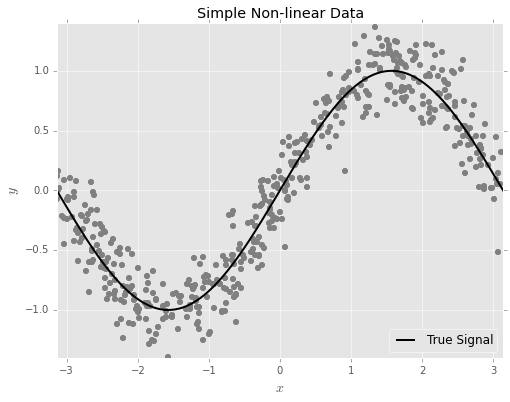
\includegraphics[scale=0.50]{sin-with-data}
    \end{figure}
   }
   \only<2>{
    \begin{figure}
      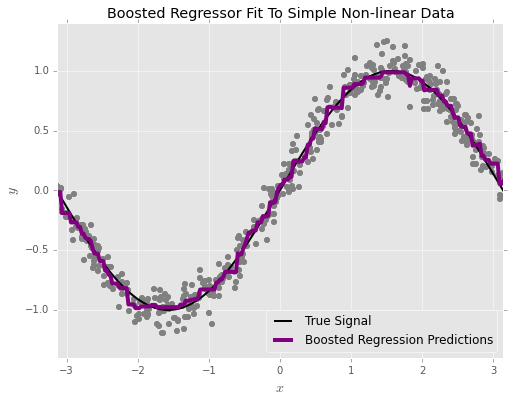
\includegraphics[scale=0.50]{sin-with-data-and-booster}
    \end{figure}
   }
   \only<3>{
    \begin{figure}
      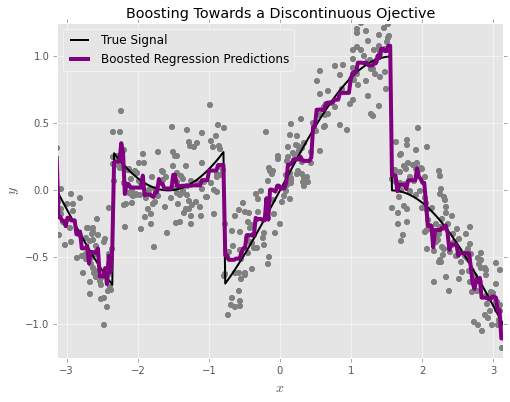
\includegraphics[scale=0.50]{broken-sin-with-booster}
    \end{figure}
   }
\end{frame}
%
\begin{frame}
Boosting accomplishes this by \textit{growing the model gradually}
  \begin{figure}
    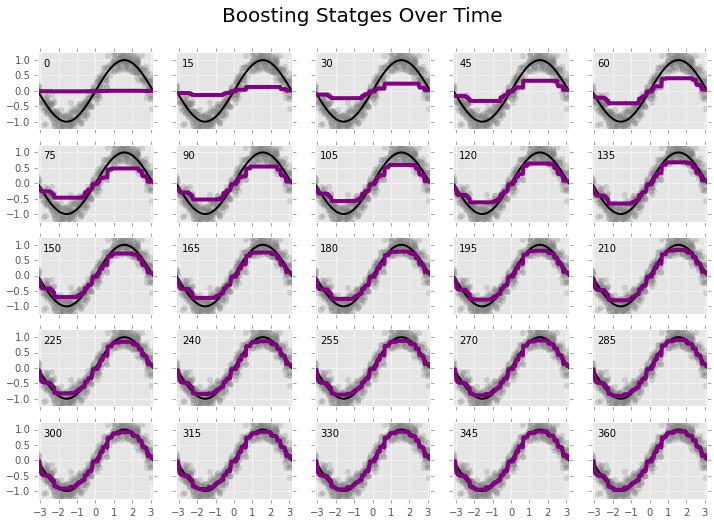
\includegraphics[scale=0.40]{boosting-over-time-multiple-plots}
  \end{figure}
\end{frame}
%
\begin{frame}
At each stage of the growth, the next model is built as an adjustment to the previous model
  \begin{figure}
    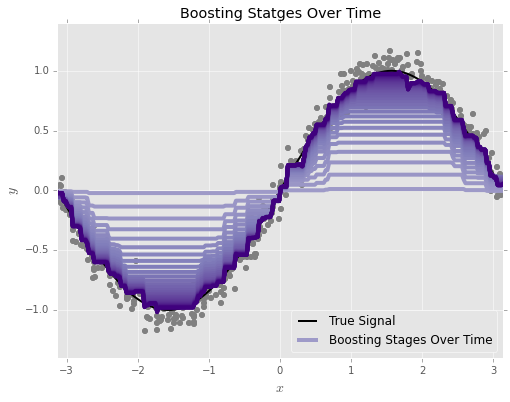
\includegraphics[scale=0.50]{boosting-over-time-single-plot}
  \end{figure}
\end{frame}
%
\begin{frame}

\only<2->{  
\textbf{Compared to}:\\~\\
}

\only<1>{
\textbf{Boosting}: \\~\\
Lowers variance by growing the model slowly over time (along with a few other tricks).\\~\\

Lowers bias by stacking many non-parametric models into the final result.
}

\only<2>{
\textbf{Linear Models}: \\~\\
Lowers variance by using a regularization penalty.\\~\\

Lowers bias by including more features.
}

\only<3>{
\textbf{SVM}: \\~\\
Lowers variance by maximizing the margin between positive and negative cases.\\~\\ 

Lowers bias by using a kernel, which projects the data into a very high dimensional space.
}

\only<4>{
\textbf{Random Forest}: \\~\\

Lowers variance by growing many learners on different subsamples of the data and predictors, then averaging them.\\~\\

Lowers bias by growing really big trees.
}

\end{frame} % Introduction
\section{Outline of the Lesson}
%
\begin{frame}
\textbf{Agenda:}
 
  \begin{itemize}
    \item Introduction
    \item You Could Have Invented Gradient Boosting
    \item Practical Gradient Boosted Regression
    \item Interpreting Gradient Boosted Regression
    \item Boosting for Classification.
    \item Drawbacks of Boosting
  \end{itemize}

\end{frame}
%
\begin{frame}
\textbf{Objectives:}

  \begin{itemize}
    \item Understand the conceptual foundation of Boosting
    \item Understand the algorithm's hyperparameters, and how to tune them.
    \item Understand some basic strategies for interpreting a booster.
    \item Understand the drawbacks of boosting.
    \item Be aware of the possibility of creating your own loss function.
  \end{itemize}
  
\end{frame} % Outline and Goals
\section{You Could Have Invented Gradient Boosting}
%
\begin{frame}
Let's start with our usual basic setup.\\~\\

$\{ x_i, y_i \}$ is a data set, where $i$ indexes the samples we have available for training our model.\\~\\

Each $x_i$ may be a vector, in which case I'll refer to it's components (if needed) as $x_{ij}$.
\end{frame}
%
\begin{frame}
Our goal is to construct a function $f$ so that

$$ y_i \approx f(x_i) \ \text{for all} \ i $$

\end{frame}
%
\begin{frame}
\textbf{Question:} What should the domain of $f$ be?
\end{frame}
%
\begin{frame}
\textbf{Degenerate Choice:} 

$$\text{Domain}(f) = \{x_i\}$$.

That is, let's only attempt to define $f$ on our training samples.
\end{frame}
%
\begin{frame}
\begin{center}
"But Matt.  This is silly.  The answer is obvious."
\end{center}

$$ \textbf{Define:} \ f(x_i) = y_i $$
\end{frame}
%
\begin{frame}
\textbf{True}.\\~\\

But let's try to derive this in a creative way.
\end{frame}
%
\begin{frame}

\only<1>{
\textbf{Recall}: Gradient descent is a general purpose algorithm for optimizing any objective function $L(x)$.\\~\\

  \begin{center}
    \textit{How does this go?}
  \end{center}
}

\only<2>{
\textbf{Algorithm:} Gradient Descent to Minimize a function $L$.\\~\\

\textbf{Inputs:} A function $f$.

\textbf{Outputs:} A point $x_{\text{optim}}$ that minimizes $f$. \\~\\

\begin{itemize}
  \item Compute $\nabla L(x)$ somehow, on paper is good.
  \item Initialize $x_0 = 0$ (arbitrary, there may be more principled choices).
  \item Iterate until convergence: \begin{itemize}
    \item Set $x_{i+1} = x_i - \nabla L(x_i)$.
  \end{itemize}
\end{itemize}
}

\end{frame}
%
\begin{frame}
Let's focus on a \textit{single point in our domain}, and try to minimize the classic squared error loss function

$$ L(f, y) = \frac{1}{2} (y - f)^2 $$

Here $f$ is not a function yet, it is just a number.
\end{frame}
%
\begin{frame}
Initialize $f$ to the average value of $y_i$

$$ f_0 = \frac{1}{N} \sum_i y_i $$
\end{frame}
%
\begin{frame}
Compute the gradient with respect to $f$ by hand

$$ \nabla_{f} (f, y) = \frac{\partial}{\partial f} \left( \frac{1}{2} (y - f)^2 \right) = f - y $$
\end{frame}
%
\begin{frame}
...and apply the update rule

$$ f_1 = f_0 - \nabla_{f} (f_0, y) = f_0 - (f_0 - y) = y $$
\end{frame}
%
\begin{frame}
So this (admittedly quite bizarre) application of gradient descent immediately recovers the correct solution

$$ f(x_i) = y_i $$

for every data point.
\end{frame}
%
\begin{frame}

\begin{center}
\textbf{Question:}\\~\\

What is stopping up from applying this scheme in the more realistic situation where we want to construct a function $f$ with domain $\mathbb{R}^n$ so that
\end{center}

$$ f(x_i) \approx y_i $$
\end{frame}
%
\begin{frame}
The \textbf{first step works}, we can certainly define $f_0$ to be a constant function

$$ f_0(x) = \frac{1}{N} \sum_i y_i \ \text{for all} \ x \in \mathbb{R}^n $$
\end{frame}
%
\begin{frame}
The \textbf{update step fails}.\\~\\

We cannot evaluate the gradient at any point where we have not observed a value of $y$.

$$ \nabla_f (f, y) = f - y $$
\end{frame}
%
\begin{frame}

\begin{center}
{\huge We need to extend the gradient to points where we have not observed a value of $y$.}
\end{center}

\end{frame}

%
\begin{frame}
\textbf{Fundamental Idea Of Gradient Boosting:}\\~\\

Replace the response $y$ in our dataset with the \textbf{gradient of the loss evaluated at} $y$

$$ \{x_i, \nabla_f L(f_0(x_i), y_i) \} = \{x_i, f_0(x_i) - y_i \} $$

Then, fit a model to this new \textbf{working response}.\\~\\

The \textbf{predictions from this model} can be viewed as an (approximate) extension of the gradient to all of $\mathbb{R}^n$.

\end{frame}
%
\begin{frame}
\textbf{Algorithm:} Gradient Boosting to Minimize Sum of Squared Errors.\\~\\

\textbf{Inputs:} A data set $\{ x_i, y_i \}$.

\textbf{Returns:} A function $f$ such that $f(x_i) \approx y_i$.

\begin{itemize}
  \item Initialize $f_0(x) = \frac{1}{N} \sum_i y_i$.
  \item Iterate (parameter $k$) until satisfied: \begin{itemize}
    \item Create the working data set $W_k = \{ x_i, f_k(x_i) - y_i \}$.
    \item Fit a decision tree to $W_k$, minimizing least squares (though most anything would work here).  Call this tree $T_k$.
    \item Set $f_{k+1}(x) = f_{k}(x) - T_{k}(x)$. 
  \end{itemize}
  \item Return $f_{\text{max}}(x) = f_0(x) - T_1(x) - T_2(X) - \cdots - T_{\text{max}}(x)$.
\end{itemize}
\end{frame}
%
\begin{frame}
\textbf{Comments:}

\only<2->{
\begin{itemize}
  \item We didn't \textit{have} to use decision trees, literally anything would work.
}
\only<3->{
  \item Just like in other algorithms, we can introduce a \textit{learning rate} to make the gradient descent more robust
  $$ x_{i+1} = x_i - \lambda \nabla L(x_i) $$
This is particularly important in boosting, to prevent overfitting.
}
\only<4->{
  \item We could have fit the tree to the negative gradient, which would have resulted in the more aesthetically appealing
  $$ f_{\text{max}}(x) = f_0(x) + T_1(x) + T_2(X) + \cdots + T_{\text{max}}(x) $$
}
\only<2->{
\end{itemize}
}
\end{frame}




 % You Could Have Invented Gradient Boosting
%
\end{document}
